\documentclass[final,3p,times,twocolumn]{elsarticle}

%% Use the option review to obtain double line spacing
%% \documentclass[preprint,review,12pt]{elsarticle}

%% Use the options 1p,twocolumn; 3p; 3p,twocolumn; 5p; or 5p,twocolumn
%% for a journal layout:
%% \documentclass[final,1p,times]{elsarticle}
%% \documentclass[final,1p,times,twocolumn]{elsarticle}
%% \documentclass[final,3p,times]{elsarticle}
%% \documentclass[final,3p,times,twocolumn]{elsarticle}
%% \documentclass[final,5p,times]{elsarticle}
%% \documentclass[final,5p,times,twocolumn]{elsarticle}

%% if you use PostScript figures in your article
%% use the graphics package for simple commands
%% \usepackage{graphics}
%% or use the graphicx package for more complicated commands
%% \usepackage{graphicx}
%% or use the epsfig package if you prefer to use the old commands
%% \usepackage{epsfig}

%% The amssymb package provides various useful mathematical symbols
\usepackage{amssymb}
%% The amsthm package provides extended theorem environments
%% \usepackage{amsthm}
%% The bm package lets you access bold symbols in math mode using the \boldsymbol command (useful to get bold greek letters).
\usepackage{bm}
%% The bbm package is contains the indicator function symbol \mathbbm{1}
\usepackage{bbm}
%% The amsmath package contains the split environment, letting you split equations into multiple lines.
%% See "https://www.sharelatex.com/learn/Aligning_equations_with_amsmath " for an explanation.
\usepackage{amsmath}
%% The lineno packages adds line numbers. Start line numbering with
%% \begin{linenumbers}, end it with \end{linenumbers}. Or switch it on
%% for the whole article with \linenumbers after \end{frontmatter}.
%% \usepackage{lineno}
%% The algorithm defines the algorithm floating environment and the algpseudocode package is useful for constructing Pseudo code.
\usepackage{algorithm}
\usepackage{algpseudocode}
%% For creating pictures
\usepackage{tikz}

%% Declaring \argmin and \argmax operators:
\DeclareMathOperator*{\argmin}{arg\,min}
\DeclareMathOperator*{\argmax}{arg\,max}
%% Declare trace operator \Tr:
\DeclareMathOperator*{\Tr}{Tr}
%% Declare pdf functions
\DeclareMathOperator*{\Dir}{Dir}
\DeclareMathOperator*{\DP}{DP}
%% shorthand for \boldsymbol
\let\bs\boldsymbol
%% natbib.sty is loaded by default. However, natbib options can be
%% provided with \biboptions{...} command. Following options are
%% valid:

%%   round  -  round parentheses are used (default)
%%   square -  square brackets are used   [option]
%%   curly  -  curly braces are used      {option}
%%   angle  -  angle brackets are used    <option>
%%   semicolon  -  multiple citations separated by semi-colon
%%   colon  - same as semicolon, an earlier confusion
%%   comma  -  separated by comma
%%   numbers-  selects numerical citations
%%   super  -  numerical citations as superscripts
%%   sort   -  sorts multiple citations according to order in ref. list
%%   sort&compress   -  like sort, but also compresses numerical citations
%%   compress - compresses without sorting
%%
%% \biboptions{comma,round}

% \biboptions{}


\journal{MPhil in Scientific Computing}

\begin{document}

\begin{frontmatter}

%% Title, authors and addresses

%% use the tnoteref command within \title for footnotes;
%% use the tnotetext command for the associated footnote;
%% use the fnref command within \author or \address for footnotes;
%% use the fntext command for the associated footnote;
%% use the corref command within \author for corresponding author footnotes;
%% use the cortext command for the associated footnote;
%% use the ead command for the email address,
%% and the form \ead[url] for the home page:
%%
%% \title{Title\tnoteref{label1}}
%% \tnotetext[label1]{}
%% \author{Name\corref{cor1}\fnref{label2}}
%% \ead{email address}
%% \ead[url]{home page}
%% \fntext[label2]{}
%% \cortext[cor1]{}
%% \address{Address\fnref{label3}}
%% \fntext[label3]{}

\title{Mini Project: Dirichlet Processes and the Dirichlet Process Mixture}

%% use optional labels to link authors explicitly to addresses:
%% \author[label1,label2]{<author name>}
%% \address[label1]{<address>}
%% \address[label2]{<address>}

\author{Brian Azizi}

\address{Cavendish Laboratory, Department of Physics, J J Thomson
  Avenue, Cambridge. CB3 0HE}

\begin{abstract}
As part of the written assignment for the MPhil in Scientific Computing, we have implemented three clustering algorithms in the C++ programming language: the k-means algorithm, the Gaussian mixture model and the Dirichlet Process mixture model.
Subsequently, the algorithms will be compared and texted on a number of data sets.
\end{abstract}

\end{frontmatter}

%%
%% Start line numbering here if you want
%%
% \linenumbers

%% main text
\section{Introduction}
\label{sect:Intro}
In this written assignment, we introduce the \emph{Dirichlet Process Mixture (DPM)} as a \emph{non-parametric Bayesian} model for clustering.
We begin with a general discussion of Dirichlet Processes (DP).
We then give four different representations of DPs that give us a deeper intuitive understanding in section \ref{sect:representation}.
Section \ref{sect:DPM} explains how Dirichlet processes can be applied to clustering via the Dirichlet Process Mixture.
Following this, we discuss inference in the DPM and our implementation of the model.
Here, we will also give some output of our implementation.
In the final section, we discuss further work and conclude.

\section{Bayesian Parametrics and the Dirichlet Distribution}
In this section, we describe the Dirichlet distribution.

\subsection{Discrete Random Variables and the Categorical Distribution}
Consider a discrete random variable $x$ that can take one of $K$ possible categorical values, $x \in \{1,\dots,K\}$.
The distribution of $x$ is then fully specified by the probabilities $\pi_k = P(x = k)$ and its probability mass function (pmf) is given by
\begin{equation}
\label{eqn:catpmf}
p(x\,|\,\pi_1,\dots,\pi_K) = \prod_{k=1}^K \pi_k^{\,\delta_{x,k}}
\end{equation}
where we made use of the Kronecker delta defined by
\begin{equation}
\label{eqn:kronecker}
\delta_{i,j} := \mathbbm{1}\{i = j\} = \left\{\begin{array}{lr}
1 & \mbox{if $i = j$}\\
0 & \mbox{otherwise} \end{array} \right.
\end{equation}

We say that $x$ follows the \emph{categorical distribution}
\footnote{This distribution is sometimes also referred to as the \emph{Discrete}, the \emph{Multinoulli} or (somewhat inaccurately) the \emph{Multinomial} distribution.}
, denoted $x \sim Cat(\pi_1, \dots, \pi_K)$.
This can be viewed as a generalization of the Bernoulli distribution to more than two outcomes.
Alternatively, we can specify the distribution of $x$ through a \emph{(generalized) probability density function (pdf)} by making use of the \emph{Dirac delta function}.
\footnote{The Dirac delta can be loosely thought of as a function on $\mathbb{R}$ which is zero everywhere except at the origin where it is infinite,
\[\delta(x) = \left\{
\begin{array}{ll}
+\infty, & x = 0\\
0, & \mbox{otherwise}
\end{array} \right.\]
and whose integral over the real line is unity
\[ \int_{-\infty}^{+\infty}\delta(x)dx = 1.\]
Note however, that this is not a formal definition. $\delta$ can be rigorously defined using measure theory or the theory of generalized functions.}

\begin{equation}
\label{eqn:catpdf}
f(x) = \sum_{k=1}^K \pi_k \delta(x - k)
\end{equation}

Generalized probability density functions greatly unify the analysis of discrete and continuous random variables (as well as variables that are discrete on some parts of the probabiliy space and continuous on others).
For instance, the usual definitions of expectation, variance, etc for continuous variables can be directly carried over to the case of discrete variables.
In this context, points in probability space with non-zeros probability mass are referred to as \emph{atoms} (thus, the pdf of categorical variables consists entirely of atoms).
Figure \ref{fig:pmf} illustrates the pdf of $x$.

\begin{figure}
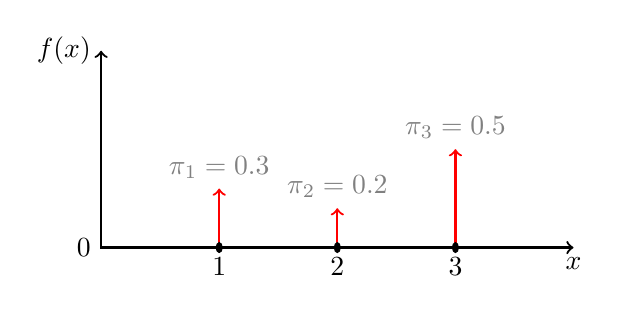
\begin{tikzpicture}[yscale=2.5,xscale=1.5]
\draw[thick,<->] (0,1) node [left] {$f(x)$} -- (0,0) node [left] {$0$} -- (4,0) node [below] {$x$};
\draw[red,thick,->] (1,0) -- (1,0.3) node [above,gray] {$\pi_1 = 0.3$};
\draw[red,thick,->] (2,0) -- (2,0.2) node [above,gray] {$\pi_2 = 0.2$};
\draw[red,thick,->] (3,0) -- (3,0.5) node [above,gray] {$\pi_3 = 0.5$};
\draw[fill] (1,0) circle [radius=0.025] node [below] {$1$};
\draw[fill] (2,0) circle [radius=0.025] node [below] {$2$};
\draw[fill] (3,0) circle [radius=0.025] node [below] {$3$};
\end{tikzpicture}
\caption{The probability density function of a discrete random variable that can occupy 3 possible states ($K=3$).}
\label{fig:pmf}
\end{figure}

In order for the pmf and the pdf of the categorical distribution to be well-defined, we require that $\pi_k \geq 0$ and $\sum_{k=1}^K \pi_k = 1$ since the $\pi_k$ represent probabilities.
In other words, we require $\bs \pi = (\pi_1,\dots,\pi_K)$ to live on the \emph{$K$-dimensional probability simplex}
\footnote{Note however that, due to the sum-to-one constraint, $\Delta_K$ is in fact only a $(K-1)$-dimensional manifold embedded in $K$-dimensional Euclidean space.
For this reason, some authors refer to $\Delta_K$ as the $(K-1)$-dimensional probability simplex (and use the notation $\Delta_{K-1}$ instead).}
defined as
\begin{equation}
\label{eqn:simplex}
\Delta_K = \left\{(\pi_1,\dots,\pi_K) \in \mathbb{R}^K : \pi_k \geq 0,\,\, \sum \nolimits _{k=1}^K \pi_k = 1\right\}.
\end{equation}
Figure \ref{fig:simplex} depicts $\Delta_K$ when $K=3$.

\begin{figure}
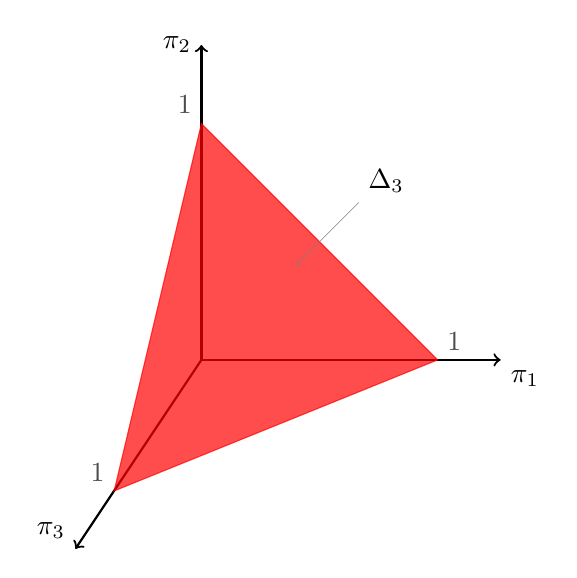
\begin{tikzpicture}[scale=2]
\draw[thick,<-] (0,2) node [left] {$\pi_2$} -- (0,0);
\draw[thick,->] (0,0) -- (1.9,0) node [below right] {$\pi_1$};
\draw[thick,->] (0,0) -- (-0.8,-1.2) node [above left] {$\pi_3$};
\draw[red, fill=red, opacity=0.7] (1.5,0) node [above right, black] {$1$} -- (0,1.5) node [above left, black] {$1$} -- (-.554,-.832) node [above left, black] {$1$} -- (1.5,0);
\draw[help lines,<-] (0.6,0.6) -- (1,1) node [above right, black] {$\Delta_3$};
\end{tikzpicture}
\caption{The 3-dimensional probability simplex $\Delta_3$.}
\label{fig:simplex}
\end{figure}

Now suppose we have a dataset $S=\{x_{(i)}\}_{i=1}^N$ consisting of $N$ independent observations of $x$.
The corresponding likelihood function takes the form
\begin{equation}
\label{eqn:catlik}
\begin{split}
p(S\,|\,\bs \pi) &= \prod_{i=1}^N \prod_{k=1}^K \pi_k^{\delta_{x^{(i)},k}} \\ &= \prod_{k=1}^K \pi_k^{\left(\sum_{i=1}^N \delta_{x^{(i)},k}\right)} = \prod_{k=1}^K \pi_k^{\,m_k}
\end{split}
\end{equation}
where $m_k = \sum_{i=1}^N \delta_{x^{(i)}, k}$ represents the number of observation in which $x$ takes the value $k$.
The quantities $m_k$ are the sufficient statistics of the categorical distribution.

\subsubsection*{\normalfont \small \bfseries Maximum Likelihood Inference}
In the frequentist setting, we typically infer the parameter $\bs \pi$ through maximum likelihood estimation.
Given dataset $S$, we choose $\bs \pi$ that maximises the log of the likelihood function $p(S\,|\,\bs \pi)$ taking into account the constraint that $\bs \pi \in \Delta_K$.
To perform the constrained optimization, we use the method of Lagrange multipliers. We form the Lagrangian
\footnote{Generally speaking, we should include the inequality constraints $\pi_k \geq 0$ in the Lagrangian and perform the optimization via the Karush-Kuhn-Tucker conditions.
In our case we may safely ignore these constraints since our solution (equation \ref{eqn:catML}) happens to satisfy them regardless.}
using equation \ref{eqn:catlik}

\begin{equation}
\label{eqn:catlagrange}
\begin{split}
L(\bs \pi, \lambda) &= \log p(S\,|\,\bs \pi) + \lambda\left(1 - \sum \nolimits_{k=1}^K \pi_k\right)\\
&= \sum\nolimits_{k=1}^K m_k \log \pi_k + \lambda\left(1-\sum\nolimits_{k=1}^K \pi_k\right)
\end{split}
\end{equation}

Setting the derivate of $L$ with respect to the Lagrange multiplier $\lambda$ to zero, we get our sum-to-one constraint
\begin{equation}
\label{dldlambda}
\frac{\partial L}{\partial \lambda} = 1 - \sum\nolimits_{k=1}^K = 0.
\end{equation}
Differentiating with respect to $\pi_k$ gives
\begin{equation}
\frac{\partial L}{\partial \pi_k} = \frac{m_k}{\pi_k} - \lambda
\end{equation}
and setting the derivative to zero yields

\begin{equation}
\label{dldpi}
\begin{split}
\lambda \pi_k &= m_k\\
\Rightarrow \lambda \sum\nolimits_k \pi_k &= \sum\nolimits_k m_k\\
\Rightarrow \lambda &= N
\end{split}
\end{equation}

Therefore, the maximum likelihood solution is 
\begin{equation}
\label{eqn:catML}
\pi_k = \frac{m_k}{N}
\end{equation}
which is simply the fraction of observations in which $x = k$.

\subsection{The Dirichlet Distribution and Bayesian Inference}
\label{sect:dirdistro}
\begin{figure*}
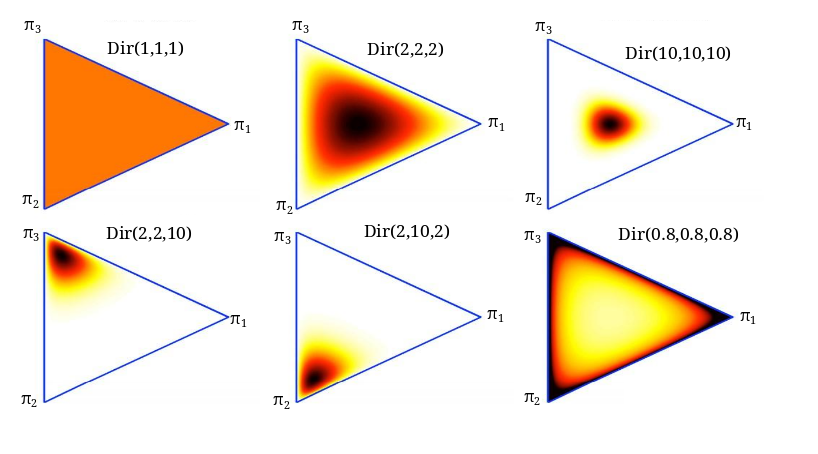
\includegraphics[width=\textwidth,height=4in]{dir.png}
\caption{Examples of Dirichlet distributions on $\Delta_3$. (Figure from \cite{ywt07})}
\label{fig:dir}
\end{figure*}

If our dataset is small (e.g. $N < K$), the maximum likelihood approach might (incorrectly) estimate many of the parameters to be zero.
Based on this analysis, we would conclude that the probability of a new sample $x^{(N+1)}$ taking on certain values to be zero.
This is sometimes referred to as the \emph{zero count problem}.

In this section, we give a quick discussion on Bayesian inference for our categorical variable $x$. Along the way, we will introduce the Dirichlet distribution and demonstrate how the Bayesian framework is less prone to the zero count problem.

In a Bayesian framework, we need to specify a prior distribution $p(\bs \pi)$for our model parameters $\bs \pi$. We then use our dataset $S$ to update the prior and obtain a posterior distribution $p(\bs \pi\,|\,S)$ for $\bs \pi$.
The update is done in accordance with Bayes rule
\begin{equation}
\label{eqn:bayes}
p(\bs \pi \,|\, S) = \frac{p(S\,|\,\bs \pi) p(\bs \pi)}{\int_{\bs \pi} p(S\,|\,\bs \pi)p(\bs \pi)d\bs\pi}.
\end{equation}
In general, the integral in the denominator is analytically intractable and numerical approximations can be very computationally intensive.
However, for some likelihood models, we can find a parametric family of distributions such that the prior and the posterior are both members of that family. 
The prior is then said to be \emph{conjugate} to the likelihood function and the parameters of the conjugate family are referred to as \emph{hyper-parameters}.
If we have conjugacy, computing the posterior is simply a matter of updating the hyper-parameters.

\subsubsection*{\normalfont \small \bfseries Dirichlet Distributions}
Looking at equation \ref{eqn:catlik} we see that the conjugate prior to a categorical likelihood function needs to have support over the probability simplex $\Delta_K$ and have a pdf of the form 
\begin{equation}
p(\bs \pi) \propto \prod\nolimits_{k=1}^K \pi_k^{\hat\alpha_k}.
\end{equation}
The Dirichlet distribution satisfies both criteria. 
It has support over the probability simplex $\Delta_K$ and its pdf
\footnote{
$\Gamma(t)$ is the \emph{Gamma function} defined as 
\[
\Gamma(t) = \int\nolimits_{-\infty}^{\infty} x^{t-1} e^{-x} dx
\]	
for $t \in \mathbb{R}_+$.
It is a generalization of the factorial function to the positive real line since for $n\in \mathbb{N}$, $\Gamma(n) = (n-1)!$.
}
is defined as
\begin{equation}
\label{eqn:dirpdf}
\Dir(\bs \pi\,|\,\bs \alpha) = \mathbbm{1}\{\bs \pi \in \Delta_K\}\frac{\Gamma(\sum_{k=1}^K\alpha_k)}{\prod_{k=1}^K\Gamma(\alpha_k)}\prod\nolimits_{k=1}^K\pi_k^{\alpha_k - 1} 
\end{equation}
The quantities $(\alpha_1,\dots,\alpha_K)$ are the \emph{concentration parameters} of the distribution and we require them to be strictly positive real numbers. 
Figure \ref{fig:dir} shows heat plots of the dirichlet pdf over $\Delta_3$ for different parameter values $\bs \alpha$.
When $\alpha_k = 1$ for all values of $k$ we get the uniform distribution.
If $\alpha_k  > 1$ we get a unimodal distribution where the position of the peak depends on the relative sizes of the $\alpha_k$ and the size of the peak depends on the magnitudes of the $\alpha_k$.
For $\alpha_k < 0$, the distribution is unbounded, multimodal and the probability mass concentrates on the edge of the simplex.

Define $\alpha_0 = \sum_{k=1}^K \alpha_k$. To work out the mean of a Dirichlet distributed variable, we first find the mean of the first component $\pi_1$,
\begin{equation}
\label{eqn:dirmean1}
\begin{split}
\mathbbm{E}\left[\pi_1\right] &= \frac{\Gamma(\alpha_0)}{\prod_{k=1}^K\Gamma(\alpha_k)} \int\nolimits_{S_K} \pi_1 \Dir(\bs \pi \,|\, \bs \alpha)d\bs\pi \\
&= \frac{\Gamma(\alpha_0)}{\prod_{k=1}^K\Gamma{\alpha_k}} \left[\int_0^1\int_0^{1-\pi_1}\dots\int_0^{1-\sum_{k=1}^{K-1}} \right.\\
& \left.\pi_1^{\alpha_1}\pi_2^{\alpha_2-1}\dots\pi_K^{\alpha_K-1}d\alpha_K \dots d\alpha_1\right]\\
&= \frac{\Gamma(\alpha_0)}{\prod_{k=1}^K\Gamma(\alpha_k)} \frac{\Gamma(\alpha_1+1)\prod_{k=2}^K\Gamma(\alpha_k)}{\Gamma(\alpha_0+1)}\\
&= \frac{\Gamma(\alpha_0)}{\prod_{k=1}^K\Gamma(\alpha_k)} \frac{\alpha_1\prod_{k=1}^K\Gamma(\alpha_k)}{\alpha_0 \Gamma(\alpha_0)}\\
&= \frac{\alpha_1}{\alpha_0}
\end{split}
\end{equation}
where we used the fact that the integral is the normalization constant of the $\Dir(\alpha_1+1,\alpha_2,\dots,\alpha_K)$ pdf in the third line and the property of the Gamma function that $\Gamma(t+1)=t\Gamma(t)$ in the fourth line. 
The derivation is symmetric for the remaining components of $\bs \pi$, thus 
\begin{equation}
\label{eqn:dirmean}
\mathbbm{E}\left[\bs \pi \right] = \frac{\bs \alpha}{\alpha_0}
\end{equation}

Often, a symmetric Dirichlet distribution of the form $\alpha_k = \alpha \forall k$ is used as prior.
In this case, the mean of the $k$th component of $\pi_k$ is $\mathbbm{E}\left[\pi_k\right] = 1/K$.
It can be shown that the variance of $\pi_k$ is given by
\begin{equation}
\label{eqn:dirvar}
\mathbb{V}\left[\pi_k\right] = \frac{K-1}{K^2(\alpha K + 1)}.
\end{equation}
In this case, $\alpha$ corresponds to the inverse variance of the distribution.

\subsubsection*{\normalfont \small \bfseries Conjugate Bayesian Inference of Categorical Variables}
Previously, we had $x \sim Cat(\pi_1,\dots,\pi_K)$ and a dataset $S = \{x^{(i)}\}_{i=1}^N$. Suppose we give $\bs \pi$ a Dirichlet prior: $\bs \pi \sim \Dir(\bs \alpha)$. 
From equation \ref{eqn:bayes}, we know that the posterior pdf, $p(\bs \pi \,|\, S)$ of $\bs \pi$ is proportional to the likelihood function $p(S\,|\,\bs \pi)$ times the prior pdf $p(\bs \pi)$.
Thus, from equations \ref{eqn:catlik} and \ref{eqn:dirpdf}, we get
\begin{equation}
\label{eqn:dirpost}
\begin{split}
p(\bs \pi \,|\, S) &\propto \prod\nolimits_{k=1}^K\pi_k^{m_k} \prod\nolimits_{k=1}^K \pi_k^{\alpha_k - 1}\\
	&= \prod\nolimits_{k=1}^K \pi_k^{\alpha_k+m_k-1}
\end{split}
\end{equation}
and we recognize this as the pdf of a Dirichlet distribution with parameter vector $(\alpha_1+m_1,\dots,\alpha_K+m_K) = \bs \alpha + \bs m$.

The \emph{posterior predictive distribution} of our model (that is, the distribution that a new sample $x^{(N+1)}$ would have, conditional on the observed data $S$) is obtained by marginalising out the model parameters $\bs \pi$ over the posterior distribution:
\begin{equation}
\begin{split}
p(X = k\,|\,S) &= \int p(X = k\,|\,\bs \pi)p(\bs \pi \,|\,S)d\bs\pi\\
&= \int p(X = k\,|\,\pi_k)\left[\int p(\bs \pi_{-k},\pi_k\,|\,S)d\bs\pi_{-k}\right]d\pi_k\\
&= \int \pi_k p(\pi_k\,|\,S)d\pi_k\\
&= \mathbb{E}\left[\pi_k\,|\,S\right]\\
&= \frac{\alpha_k + m_k}{\sum_j (\alpha_j+m_j)} = \frac{\alpha_k+m_k}{\alpha_0 + N}
\end{split}
\end{equation}
where we use $\bs \pi_{-k}$ to denote all components of $\bs \pi$ except $\pi_k$.

Note that this method of prediction circumvents the zero count problem.
We also see that we may interpret the hyperparameters as \emph{pseudo data}.
$\alpha_0$ is the effective size of the pseudo data set and $\alpha_k$ is the effective number of times that $x$ takes on value $k$ in the pseudo data.
The posterior distribution of $\bs \pi$ takes into account both our prior believe about $x$ (via the pseudo data) and the actual observed data.

\section{The Dirichlet Process}
\label{sect:dp}
Having discussed the Dirichlet distribution and its role in the parametric Bayesian analysis of discrete random variables, we are now ready to explore the Dirichlet process and its role in Bayesian nonparametrics.
In this section, we will first give an informal description of the Dirichlet process and show how draws from a Dirichlet process can be visualized.
We then give a formal mathematical definition of the DP and discribe its parameters.

\subsubsection*{\normalfont \small \bfseries From the Dirichlet Distribution to the Dirichlet Process}
We saw that the Dirichlet distribution can be used as a prior for categorical variables when the number of possible states $K$ is finite and known. Draws from a Dirichlet distribution give us a probability vector $\bs \pi$ of length $K$. For this reason, we can think of the Dirichlet distribution as a distribution over distributions.

The Dirichlet Process is the non-parametric extension of the Dirichlet distribution.
Instead of a random vector $\bs \pi$, a draw from a Dirichlet process is a \emph{random function} $G$ with certain properties.
And analogously to $\bs \pi$ being a valid probability distribution (since $\bs \pi$ lives on the probability simplex $\Delta_K$), $G$ is a valid probability function, a so-called \emph{probability measure}.
A probability measure is a (set) function that maps subsets from some probability space $\Omega$ onto the unit interval $[0,1]$ and that satisfies certain properties.
The most notable properties are that $G(\emptyset)=0$, $G(\Omega)=1$ and if $A_1,A_2,\dots$ are pairwise disjoint subsets of $\Omega$ (meaning $A_i\cap A_j = \emptyset$ if $i\neq j$), then $G(\cup_{i=1}^\infty A_i) = \sum_{i=1}^\infty G(A_i)$.
\footnote{There are also conditions on the domain of a measure.
The collection of subsets of $\Omega$ on which a measure is defined is called a \emph{$\sigma$-algebra} of $\Omega$.
A $\sigma$-algebra must contain the empty subset, be closed under complement and be closed under union or intersection of countably many subsets.}

In the parametric case, our categorical variable $x$ could take on an integer between $1$ and $K$.
Thus, our probability space in that case was $\Omega = \{1,\dots,K\}$.
In equation \ref{eqn:catpdf} we defined a probability density for $x$.
It is also possible to define a probability measure $\mu$ on $A \subset \Omega$ using the \emph{Dirac measure} defined by
\footnote{This is the third $\delta$-type object we have introduced in this document.
Both the Kronecker delta and the Dirac delta function can be thought of as special cases of the Dirac measure.}
\begin{equation}
\label{eqn:diracmeasure}
\delta_x(A) = \left\{ \begin{array}{lr}
1 & \mbox{if $x \in A$} \\
0 & \mbox{otherwise}
\end{array} \right.
\end{equation}
The measure $\mu$ can then be expressed as 
\begin{equation}
\label{eqn:discretemeasure}
\mu(A) = \sum\nolimits_{k=1}^K \pi_k \delta_x (A)
\end{equation}
and is known as the \emph{discrete measure}. 

In the case of the Dirichlet process, the $\Omega$ can be any general valid probability space (not necessarily finite or even countable) and $G$ can be any probability measure on $\Omega$.
If we have a random variable $\theta$ that takes values in $\Omega$, then the measure $G$ induces a probability distribution for $\theta$.
If $A$ is measurable subset of $\Omega$, we can define $Pr(\theta \in A) = G(A)$.
%However, it turns out that draws from a Dirichlet process are discrete measures on $\Omega$ almost surely (i.e. with probability one).

\subsubsection*{\normalfont \small \bfseries A mathematical definition of the Dirichlet process}
Let $A_1,\dots,A_K$ be a finite partition of $\Omega$.
This means $A_1 \cup \dots \cup A_K = \Omega$ and $A_k$ are pairwise disjoint.
If $G$ is a measure on $\Omega$, then $(A_k)$ is some number between $0$ and $1$ and $\sum_{k=1}^K G(A_k) = 1$.
In other words, the vector $G(A_1),\dots,G(A_K)$ lives on the probabilty simplex $\Delta_K$.
Suppose now that $G$ is randomly drawn from a Dirichlet process, $G \sim \DP$.
Then $(G(A_1),\dots,G(A_K))$ is a random vector and we can specify a distribution for it.

\begin{figure}
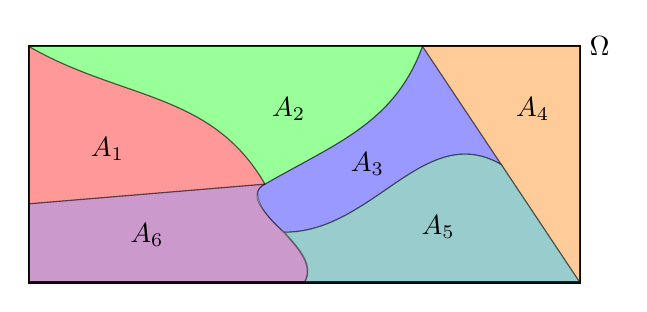
\begin{tikzpicture}[scale=1]
\draw [thick] (0,0) rectangle (7,3);
\draw [fill=red,opacity=0.4] (0,3) to [out=330, in=120] (3,1.25) to (0,1) to (0,3);
\node at (1,1.7) {$A_1$};
\draw [fill=green,opacity=0.4] (0,3) to [out=330, in=120] (3,1.25) to [out=30,in=250] (5,3);
\node at (3.3,2.2) {$A_2$};
\draw [fill=blue,opacity=0.4] (3,1.25) to [out=30,in=250] (5,3) to (6,1.5) to [out=150,in=0] (3.25,0.64) to [out=145,in=200] (3,1.25);
\node at (4.3,1.5) {$A_3$};
\draw [fill=orange,opacity=0.4] (5,3) -- (7,0) -- (7,3) -- (5,3);
\node at (6.4,2.2) {$A_4$};
\draw [fill=teal,opacity=0.4] (7,0) to (6,1.5) to [out=150,in=0] (3.25,0.64) to [out=310,in=60] (3.5,0) to (7,0);
\node at (5.2,0.7) {$A_5$};
\draw [fill=violet,opacity=0.4] (3,1.25) to [out=210,in=60] (3.5,0) to (0,0) to (0,1) to (3,1.25);
\node at (1.5,0.6) {$A_6$};
\node at (7,3) [right] {$\Omega$};
\end{tikzpicture}
\caption{A finite partition of $\Omega$.}
\label{fig:partition}
\end{figure}

The Dirichlet process is implicitly defined by the requirement that $(G(A_1), \dots, G(A_K))$ has a joint Dirichlet distribution.
We write 
\[G \sim \DP(\alpha,H)\]
if 
\begin{equation}
\label{eqn:dpdef}
(G(A_1),\dots,G(A_K)) \sim \Dir(\alpha H(A_1), \dots, \alpha H(A_K))
\end{equation}
for any finite partition $A_1,\dots,A_K$ of $\Omega$.

A Dirichlet process is specified by a \emph{concentration parameter} $\alpha$ which is a positive real number, and a \emph{base measure} $H$ which is a probability measure on the probability space $\Omega$.
Two describe the expectation and variance of Dirichlet process distributed measure $G$, consider any measurable subset $A$ of $\Omega$. 
The expectation is given by
\begin{equation}
\label{eqn:meandp}
\mathbb{E}\left[G(A)\right] = H(A)
\end{equation}
and the variance is given by
\begin{equation}
\label{eqn:vardp}
\mathbb{V}\left[G(A)\right] = \frac{H(A)(1-H(A))}{\alpha + 1}.
\end{equation}
We see that we may think of the base measure $H$ as the mean of the Dirichlet process, whereas $\alpha$ plays the role of the inverse-variance.

\section{Representations of the Dirichlet Process}
\label{sect:representations}
So far, the discussion on Dirichlet processes has been very abstract and the formal definition we gave was non-constructive and somewhat limited for practical applications. 
In this section, we will briefly review several representations of the Dirichlet process.
We will see that samples from a Dirichlet process are discrete measures and that they exhibit clustering behaviour.
to get a stronger intuition about its properties.

\subsubsection*{\normalfont \small \bfseries Posterior Dirichlet Processes}
Suppose $G$ is Dirichlet process distributed, $G \sim \DP(\alpha,H)$.
Then $G$ is a random probability measure over $\Omega$ and we may treat it as a probability distribution over $\Omega$ (we are skipping some of the measure-theoretic details).
Let $\theta$ be a sample drawn from $G$, $\theta \sim G$.
What is the prior predictive distribution of $\theta$, $p(\theta)$? Furthermore, given $\theta$, what can we say about the posterior distribution of $G$?



\section{The Dirichlet Process Mixture}
\label{sect:DPM}

See \cite{Murphy}

\section*{Acknowledgements}
Here I acknowledge the assistance of my supervisor, my industrial sponsor,
and the effects of caffine on my ability to produce this report on time.

%% The Appendices part is started with the command \appendix;
%% appendix sections are then done as normal sections
\appendix

%% References
%%
%% Following citation commands can be used in the body text:
%% Usage of \cite is as follows:
%%   \cite{key}         ==>>  [#]
%%   \cite[chap. 2]{key} ==>> [#, chap. 2]
%%

%% References with bibTeX database:
\section*{Bibliography}
\bibliographystyle{elsarticle-num}
\bibliography{references.bib}

%% Authors are advised to submit their bibtex database files. They are
%% requested to list a bibtex style file in the manuscript if they do
%% not want to use elsarticle-num.bst.

%% References without bibTeX database:

% \begin{thebibliography}{00}

%% \bibitem must have the following form:
%%   \bibitem{key}...
%%

% \bibitem{}

% \end{thebibliography}


\end{document}

%%
%% End of file `mini.tex'.